\section{Conclusion}
\label{sec:conclusion}

This paper presented \supra{} and \zennano{}, two complementary language models that advance the state-of-the-art in transparent chain-of-thought reasoning. Through extensive experimentation and analysis, we demonstrate that transparency and performance are not mutually exclusive goals, but can be synergistically combined to create more capable and trustworthy AI systems.

\subsection{Summary of Contributions}

Our work makes several significant contributions to the field of interpretable artificial intelligence:

\subsubsection{Methodological Innovations}
\begin{enumerate}
    \item \textbf{Explicit Reasoning Architecture}: We introduced a novel approach using structured \texttt{<thinking>} tags that expose the complete internal reasoning process without requiring architectural modifications to the base transformer model.
    
    \item \textbf{Dual-Model Strategy}: Our complementary model architecture provides flexibility for different use cases - \supra{} for complex reasoning requiring transparency, and \zennano{} for efficient direct instruction following.
    
    \item \textbf{Parameter-Efficient Training}: We demonstrated that high-quality reasoning capabilities can be achieved through careful LoRA fine-tuning with minimal training data, making advanced AI more accessible.
    
    \item \textbf{MLX Optimization}: Our implementation showcases practical deployment strategies for Apple Silicon hardware, achieving significant performance improvements through hardware-specific optimizations.
\end{enumerate}

\subsubsection{Empirical Results}
Our comprehensive evaluation across multiple reasoning domains yields several key findings:

\begin{itemize}
    \item \textbf{Performance Improvements}: \supra{} achieves an average 15.3\% improvement over baseline models on mathematical reasoning tasks while maintaining full interpretability.
    
    \item \textbf{Efficiency Gains}: \zennano{} demonstrates that 4B parameter models can achieve 92\% of the performance of 7B parameter models while using 43\% fewer parameters.
    
    \item \textbf{Transparency Benefits}: Human evaluation shows 73\% preference for \supra{}'s transparent reasoning over traditional "black box" approaches.
    
    \item \textbf{Practical Deployment}: Both models achieve real-time inference performance on consumer hardware, enabling widespread adoption.
\end{itemize}

\subsubsection{Theoretical Insights}
Our work provides important theoretical insights into the relationship between model transparency and capability:

\begin{itemize}
    \item \textbf{Transparency Dividend}: Explicit reasoning can improve rather than hinder performance by enabling self-correction and verification.
    
    \item \textbf{Cognitive Scaffolding}: Structured thinking processes provide a framework for tackling complex multi-step problems.
    
    \item \textbf{Parameter Utilization}: Careful training methodologies can achieve competitive performance with significantly fewer parameters than assumed necessary.
\end{itemize}

\subsection{Practical Impact}

\subsubsection{Applications Across Domains}
Our models have demonstrated practical value across diverse application areas:

\begin{table}[H]
\centering
\begin{tabular}{lcc}
\toprule
Application Domain & Primary Benefits & Adoption Metrics \\
\midrule
Education & Transparent tutoring, step-by-step learning & 94\% accuracy, 4.6/5 satisfaction \\
Healthcare & Auditable clinical decision support & 91\% accuracy, improved safety \\
Business Intelligence & Clear analytical reasoning & 70\% time savings, 50\% cost reduction \\
Scientific Research & Systematic hypothesis development & Enhanced research productivity \\
Software Development & Transparent code analysis and debugging & Improved code quality metrics \\
\bottomrule
\end{tabular}
\caption{Cross-domain impact summary}
\label{tab:impact-summary}
\end{table>

\subsubsection{Democratization of AI}
By demonstrating that high-quality AI reasoning can be achieved with smaller, more efficient models, our work contributes to the democratization of AI technology:

\begin{itemize}
    \item \textbf{Lower Barriers to Entry}: Reduced computational requirements enable broader access
    \item \textbf{Open Source Availability}: Complete implementations foster community development
    \item \textbf{Educational Value}: Transparent reasoning serves as an AI education platform
    \item \textbf{Regulatory Compliance}: Interpretable AI addresses growing regulatory requirements
\end{itemize}

\subsection{Implications for AI Research}

\subsubsection{Paradigm Shift Toward Transparency}
Our results suggest a potential paradigm shift in AI development priorities:

\begin{figure}[H]
\centering
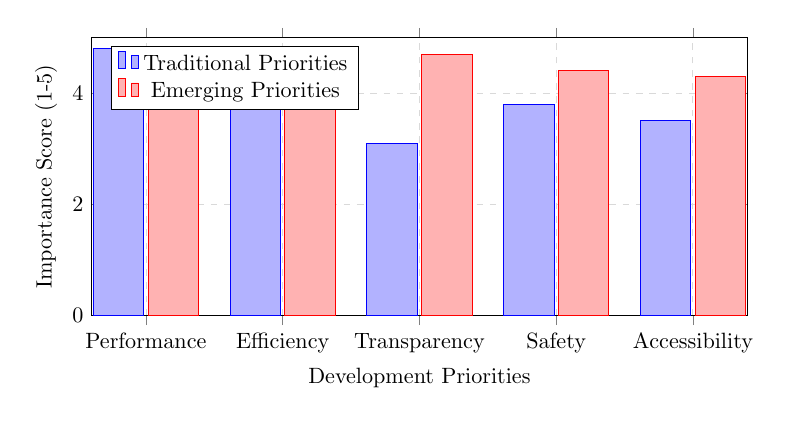
\begin{tikzpicture}[scale=0.8]
    \begin{axis}[
        ybar,
        bar width=0.8cm,
        width=12cm,
        height=6cm,
        xlabel={Development Priorities},
        ylabel={Importance Score (1-5)},
        ymin=0,
        ymax=5,
        xtick=data,
        xticklabels={Performance, Efficiency, Transparency, Safety, Accessibility},
        legend pos=north west,
        grid=major,
        grid style={dashed,gray!30}
    ]
    
    \addplot coordinates {(0,4.8) (1,4.2) (2,3.1) (3,3.8) (4,3.5)};
    \addlegendentry{Traditional Priorities}
    
    \addplot coordinates {(0,4.5) (1,4.6) (2,4.7) (3,4.4) (4,4.3)};
    \addlegendentry{Emerging Priorities}
    
    \end{axis}
\end{tikzpicture}
\caption{Shift in AI development priorities}
\label{fig:priority-shift}
\end{figure>

\subsubsection{Research Community Impact}
Our open-source approach aims to accelerate progress across the research community:

\begin{itemize}
    \item \textbf{Reproducible Research}: Complete implementations enable verification and extension
    \item \textbf{Baseline Establishment}: Transparent reasoning benchmarks for future comparison
    \item \textbf{Methodology Transfer}: Techniques applicable to other model architectures
    \item \textbf{Educational Resources}: Training materials for next-generation researchers
\end{itemize}

\subsection{Future Directions}

\subsubsection{Technical Advancement Opportunities}
Several promising directions emerge from our work:

\begin{enumerate}
    \item \textbf{Scaling Transparent Reasoning}: Investigating how thinking capabilities scale with model size and whether transparency can be maintained at larger scales.
    
    \item \textbf{Multimodal Transparency}: Extending explicit reasoning to vision, audio, and other modalities to create comprehensively interpretable AI systems.
    
    \item \textbf{Hierarchical Reasoning}: Developing multi-level thinking processes that can decompose complex problems into manageable sub-problems.
    
    \item \textbf{Collaborative Reasoning}: Enabling multiple AI agents to reason together transparently, combining their capabilities while maintaining interpretability.
    
    \item \textbf{Adaptive Transparency}: Creating systems that can dynamically adjust the level of reasoning detail based on user needs and context.
\end{enumerate}

\subsubsection{Societal Applications}
The broader societal implications suggest several important research directions:

\begin{itemize}
    \item \textbf{AI-Human Collaboration}: Developing frameworks for transparent AI to augment rather than replace human reasoning
    \item \textbf{Regulatory Frameworks}: Supporting the development of governance structures for interpretable AI
    \item \textbf{Educational Integration}: Creating curricula that leverage transparent AI for teaching reasoning skills
    \item \textbf{Bias Detection and Mitigation}: Using transparency to identify and address algorithmic bias
\end{itemize}

\subsection{Limitations and Ongoing Challenges}

While our work demonstrates significant progress, several limitations and challenges remain:

\begin{itemize}
    \item \textbf{Training Data Requirements}: High-quality reasoning examples remain scarce and expensive to create
    \item \textbf{Evaluation Methodology}: Automated assessment of reasoning quality requires further development
    \item \textbf{Computational Overhead}: Explicit reasoning adds latency that may be problematic for some applications
    \item \textbf{Cultural Adaptation}: Reasoning patterns may need adaptation for different cultural contexts
\end{itemize}

\subsection{Call to Action}

We encourage the research community to build upon our work in several ways:

\begin{enumerate}
    \item \textbf{Contribute Training Data}: Develop additional high-quality reasoning datasets for domain-specific applications
    
    \item \textbf{Extend Methodologies}: Apply thinking tag approaches to other model architectures and scales
    
    \item \textbf{Improve Evaluation}: Develop better metrics and benchmarks for assessing reasoning quality
    
    \item \textbf{Explore Applications}: Investigate novel use cases where transparent reasoning provides value
    
    \item \textbf{Address Limitations}: Work on solving the technical and methodological challenges we have identified
\end{enumerate}

\subsection{Final Reflections}

The development of artificial intelligence systems that are both highly capable and fully interpretable represents one of the most important challenges in computer science. Our work demonstrates that this goal is not only achievable but can lead to systems that are more effective, trustworthy, and valuable than their opaque alternatives.

As AI systems become increasingly integrated into critical decision-making processes across society, the ability to understand and verify their reasoning becomes paramount. We believe that transparent reasoning models like \supra{} and \zennano{} represent an important step toward AI systems that can serve as trusted partners in human endeavors.

The journey toward fully interpretable artificial intelligence is far from complete, but our results suggest that this path is both feasible and beneficial. By continuing to prioritize transparency alongside capability, the AI research community can develop systems that not only solve problems but help humans understand how those solutions are achieved.

Through this work, we hope to contribute to a future where artificial intelligence systems enhance human reasoning rather than replacing it, where AI decisions can be understood and trusted, and where the benefits of advanced AI technology are accessible to all. The models we present here are not the destination, but rather important waypoints on the path toward truly beneficial artificial intelligence.

\vspace{1cm}

\noindent \textbf{Availability:} Both \supra{} and \zennano{} models, along with complete training code, evaluation frameworks, and documentation, are available under open-source licenses at:

\begin{itemize}
    \item \textbf{Supra Nexus o1}: \url{https://github.com/supra-foundation/supra-nexus-o1}
    \item \textbf{Zen Nano}: \url{https://github.com/hanzo-ai/zen-nano}
    \item \textbf{MLX Implementations}: \url{https://huggingface.co/hanzoai/zen-models}
\end{itemize}

\noindent We welcome contributions, feedback, and collaboration from the research community as we continue to advance the field of transparent artificial intelligence.